
\documentclass{article}
\title{Math 120 Assignment 1}
\author{Isaac Winger 20167000}
\date{}
\pagenumbering{gobble}

\usepackage{graphicx}
\usepackage{amsfonts}
\graphicspath{ {./} }

\begin{document}
    \begin{enumerate}
            \addtocounter{enumi}{1}
      \item \begin{enumerate}
                    \item With the original equation, the function would be a regular absolute value function but translated right by 3 and up by 1, but with the additional absolute value on x, the function would reflect along the vertical axis at zero. This would form a ``W'' shape. This function would be $f \colon \mathbb{R} \longrightarrow \mathbb{R}_{\geq 1}$
                    \begin{figure}[h]\centering
\includegraphics[width=1.5in]{absolutevalue}\end{figure}

              \item Since whenever $g(x)$ results in zero, $g(-x)$ results in $x^{2}$ and vice-versa, the final function would be a regular parabola. This function would be $g \colon \mathbb{R} \longrightarrow \mathbb{R}_{\geq 0}$.
                    \begin{figure}[h]\centering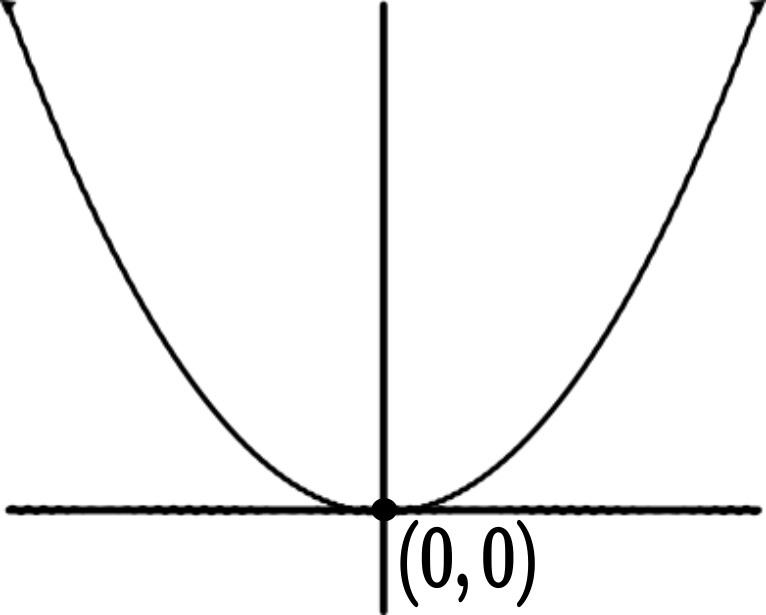
\includegraphics[width=1.5in]{parabola}\end{figure}

              \item In this equation, any value of x below three and above negative three results in an output of zero. Above three and below negative three, the equation looks like a very steep parabola with the vertexes at three and negative three. This function would be $g \colon \mathbb{R} \longrightarrow \mathbb{R}_{\geq 0}$.
              \begin{figure}[h]\centering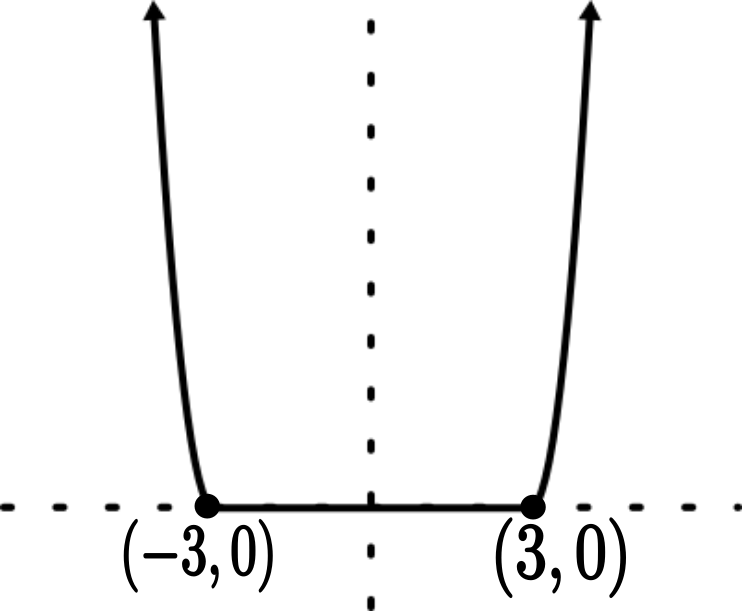
\includegraphics[width=1.5in]{polynomial}\end{figure}

                    \pagebreak

              \item No matter what x is, $h(x)$ will output either zero or one. Since both outputs are rational $h(h(x))$ will always output one. This means that the graph will look like a horizontal line at height one. This function would be $h \circ h \colon \mathbb{R} \longrightarrow \{1\}$.
              \begin{figure}[h]\centering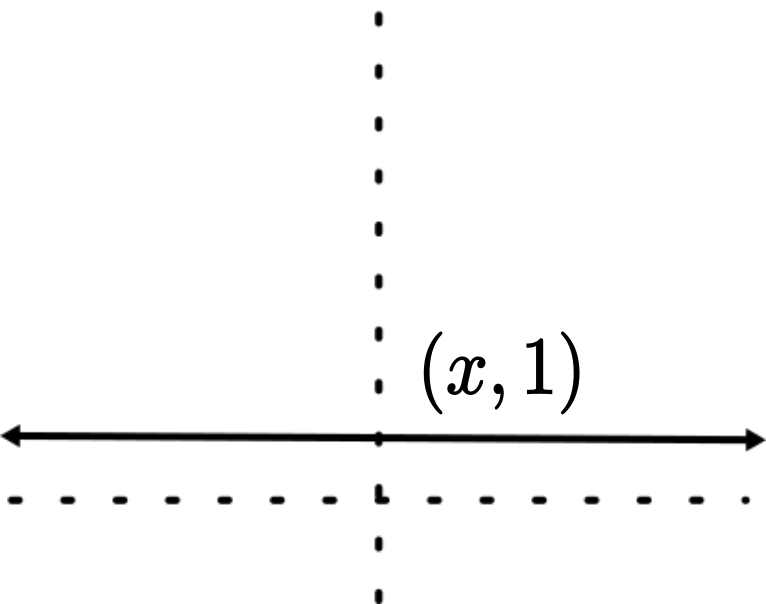
\includegraphics[width=1.5in]{line}\end{figure}



              \item There are likely infinitely many irrational numbers between any two number ranges, just as there is infinitely many rational numbers. Due to this, $h(x)$ would be constantly switching between an output of one and zero. This would give the appearance of a continuous straight line at zero, along with a continuous sin wave. The truth is that both functions would be full of tiny breaks. This function would be $h \colon \mathbb{R} \longrightarrow x \in \mathbb{R} \mid -1 \leq x \leq 1$.
              \begin{figure}[h]\centering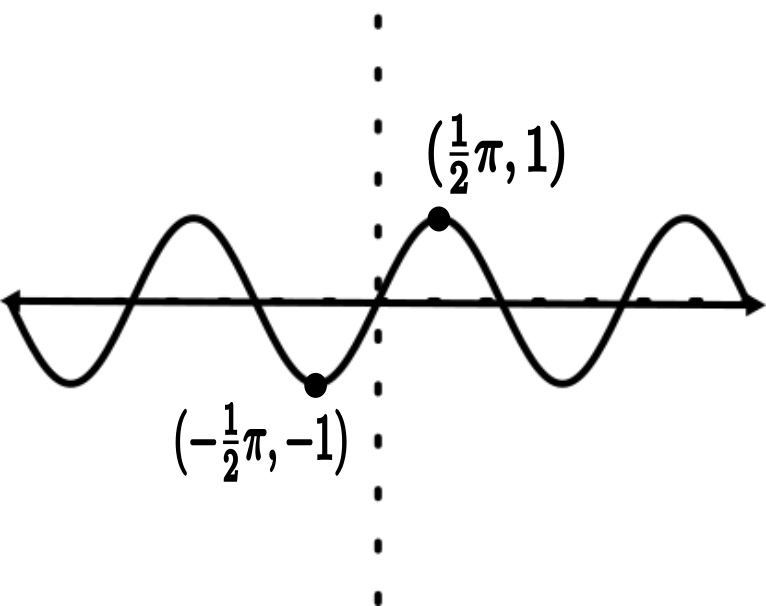
\includegraphics[width=1.5in]{sin}\end{figure}

      \end{enumerate}
\end{enumerate}
\end{document}
